\section{An overview of the Ground Handling tasks}
This section will describe which different tasks are done by the ground handling companies and how they are connected and dependent of each other.

In an interview made in Aalborg Airport with the COO, Kim Bergmann, it was found that many different airlines needs many different services and procedures done to an aircraft. There are though some most common and nearly only used tasks which will be covered in this section, but it is important to strech that any airline/ground handling company needs to be able to vairy and change these tasks since gound handling is a complex and large system. To give an overview of what tasks that are done to the aircrafts an overview of the aircraft has been made from the book Airport design and operation \cite{Airport design and operation} chapter 9 which decribes the ground handling process in detail. In graph \ref{B-777_Turnaround} we can see the different tasks done to an normal airplane during an end-station turnaround (a turnaround where passengers and luggage have arrived at their destination and new passengers, luggage and intentionally crew needs to board the flight).

\begin{figure}[H]
\centering
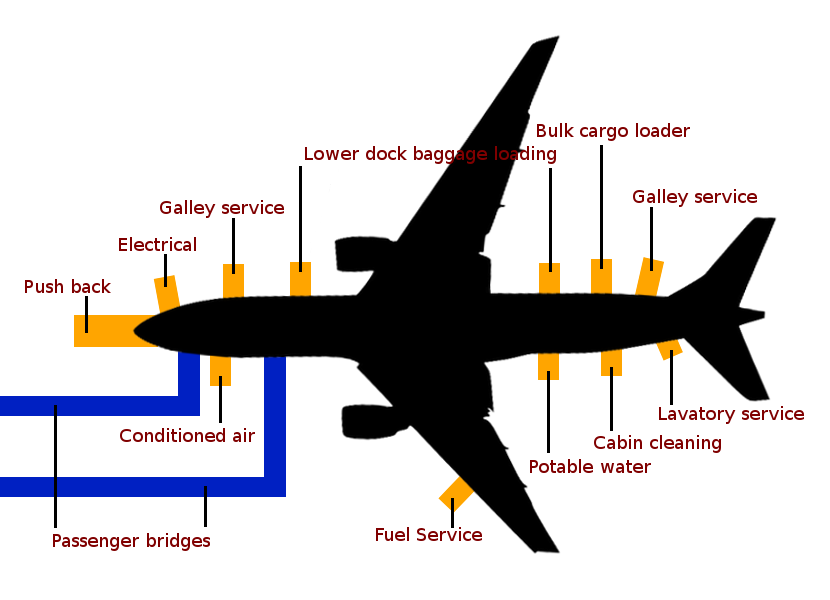
\includegraphics[width=\textwidth]{Grafik/B-777_Turnaround}
\caption{An overview of the different ground handling tasks done to an Boeing 777.http://pixabay.com/static/uploads/photo/2012/04/15/18/22/cloud-34787_640.png}
\label{B-777_Turnaround}
\end{figure}

The amount of tasks needing to be done to an airplane vary from company to company, airport to airport, time of day and ect., but this example is used to illustrate all of the categories. It is also shown where the different tasks are approximately placed on the Boeing-777, this position of cause vary from airplane to airplane and also the amount of cargo-storage areas inside the airplane and the need for either passenger bridges and/or stairs vary from airplane to airplane and also airport to airport. Also, the size of the different "vehicles" doing the tasks are not exact.

The next sections will now describe the different tasks, what they do and how they are done.

\subsection{Push back}
\subsection{Electrical}
\subsection{Galley service/catering}
\subsection{Conditioned air}
\subsection{Passenger bridges/stairs}
\subsection{Fuel service}

\subsection{Baggage and cargo loading and unloading}
\subsection{Potable water}
\subsection{Cabin cleaning}
\subsection{Lavatory service}

\section{Relationship}
Many tasks needs to done before others can start, for instance you need to unload the current luggage/cargo before new can be loaded or as described in fuel service passengers normally needs to leave the airplane before the fueling process can be started. To give a clear and structured overview the total ground handling service is divided into 3 indicidual tracks. 